In diesem Abschnitt wird die prototypische Proof-of-Concept Implementierung der \enquote{Erklärbarkeit von MMIR mittels generativer KI} beschrieben und behandelt.
Die in \cref{sec3:model} identifizierten Anwendungsfälle beschreiben die Interaktionen eines Benutzers mit dem System.
Um eine geschickte Interaktion mit dem System zu ermöglichen, wird eine Benutzungsschnittstelle mit adäquaten Interaktionsmöglichkeiten benötigt.
Die Beschreibung der Implementierung solch einer Benutzungsschnittstelle wird im Folgenden in \cref{sec4:impl:subsubsec:ui} vorgenommen.
Diese Beschreibung umfasst die Elemente der Benutzeroberfläche, sowie die Interaktion zwischen diesen.

\subsubsection{Benutzungsschnittstelle}
\label{sec4:impl:subsubsec:ui}
In diesem Abschnitt wird die Implementierung der Benutzeroberfläche beschrieben.
Für eine prototypische Proof-of-Concept Implementierung der Benutzeroberfläche wird Java's \textit{Swing} verwendet.
\textit{Swing} ist ein Werkzeug für das Erstellen von grafischen Benutzungsschnittstellen bzw. oberflächen und ist ein grundlegender Bestandteil der Laufzeitumgebung von Java.
Das Benutzen von \textit{Swing} hat somit den Vorteil, dass keine zusätzliche Installation notwendig ist und \textit{Swing} somit problemlos auf beliebigen Rechnern, auf welchen Java installiert ist, ausgeführt werden kann.
\begin{figure}[!ht]
  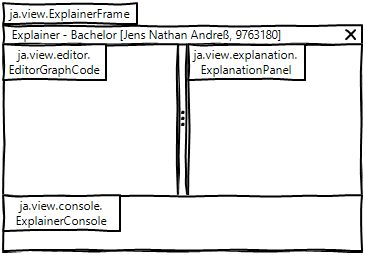
\includegraphics[width=8cm]{chapter/chapter_4/wireframe-impl-overview}
  \caption{Allgemeine Übersicht über das Mockup der Benutzungsschnittstelle.}
  \label{sec4:impl:subsubsec:ui:fig:wireframe-overview}
\end{figure}

\cref{sec4:impl:subsubsec:ui:fig:wireframe-overview} zeigt eine allgemeine Übersicht über das bereits in \cref{sec3:model:par:wireframe:fig:stage-1} vorgestellte Mockup der Benutzungsschnittstelle, erweitert um Zuweisungen der Komponenten mitsamt implementierungsspezifischen Paketnamen.
Die Elemente der in \cref{sec4:impl:subsubsec:ui:fig:wireframe-overview} gezeigten Benutzungsschnittstelle werden in \cref{sec4:impl:par:ui-elements} genauer beschrieben.
Aufbauend auf diesen Elementen wird dann in \cref{sec4:impl:par:ui-interaction} die Interaktion zwischen diesen Elementen beschrieben.
Auf diese Weise entspricht der Ablauf dieses Abschnitts dem Ablauf der Modellierung der Benutzungsschnittstelle.

\paragraph{Elemente der Benutzeroberfläche}
\label{sec4:impl:par:ui-elements}

Das Fundament der Benutzungsschnittstelle ist das \textit{ExplainerFrame}, welches durch die Klasse \textit{ja.view.ExplainerFrame} umgesetzt wird.
\cref{sec4:impl:par:ui-elements:lst:explainer-frame} zeigt die wichtigsten Aspekte der Implementierung dieser Klasse.

\lstinputlisting[style=java-code, caption={ExplainerFrame-Klasse}, label={sec4:impl:par:ui-elements:lst:explainer-frame}]{chapter/chapter_4/java/ExplainerFrame.java}

Nach der Modellierung enthält dieses Fundament drei Grundbereiche mit folgender Nummerierung (siehe \cref{sec3:model:par:wireframe:fig:stage-1}): \circitem{1} EditorGraphCode, \circitem{2} ExplainerPanel und \circitem{3} ExplainerConsole.
Diese Grundbereiche werden in \cref{sec4:impl:par:ui-elements:lst:explainer-frame} durch die privaten Variablen \textit{editorGraphCode}, \textit{explanationPanel} und \textit{explainerConsole} dargestellt.
Beim Erzeugen der Klasse \textit{ExplainerFrame} wird zuerst durch die Methode \textit{initFrame()} das Frame initialisiert und konfiguriert.
Dies umfasst die Dimension des Frames, die Position, sowie den Titel.
Darauffolgend werden dann durch die Methode \textit{initComponents()} die Komponenten, welches auch die Grundbereiche umfassen, initialisiert, konfiguriert und dem Frame hinzugefügt.
Dies umfasst besonders die notwendigen Schritte zum Hinzufügen und Layouten (z.Dt. Auslegen) der Grundbereiche im \textit{ExplainerFrame}.
Im weiteren Verlauf wird zuerst der Grundbereich \textit{EditorGraphCode}, welcher die linke Arbeitsfläche darstellt, dann der Grundbereich \textit{ExplanationPanel}, welcher die rechte Arbeitsfläche darstellt und schlussendlich der Grundbereich \textit{ExplainerConsole}, welcher die Konsole darstellt, behandelt.
Jeder dieser Grundbereiche wird mitsamt seiner enthaltenen Komponenten ausführlich behandelt, bevor mit dem nächsten Grundbereich fortgefahren wird.

\begin{figure}[!ht]
  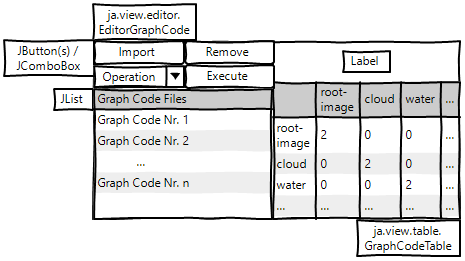
\includegraphics[width=10cm]{chapter/chapter_4/wireframe-impl-left}
  \caption{Grundbereich \textit{EditorGraphCode}.}
  \label{sec4:impl:subsubsec:ui:fig:wireframe-editor-graph-code}
\end{figure}

\cref{sec4:impl:subsubsec:ui:fig:wireframe-editor-graph-code} zeigt den Grundbereich \textit{EditorGraphCode}, umgesetzt durch die Klasse \textit{ja.view.editor.EditorGraphCode}, in welchem Benutzer durch geeignete Interaktionsmöglichkeiten die Bearbeitung von Graph Code Dateien durchführen können.
\cref{sec4:impl:par:ui-elements:lst:editor-graph-code-p1,sec4:impl:par:ui-elements:lst:editor-graph-code-p2,sec4:impl:par:ui-elements:lst:editor-graph-code-p3,sec4:impl:par:ui-elements:lst:editor-graph-code-p4} zeigen im Folgenden die wichtigsten Aspekte der Implementierung dieser Klasse.

\lstinputlisting[style=java-code, caption={EditorGraphCode-Klasse}, label={sec4:impl:par:ui-elements:lst:editor-graph-code-p1}]{chapter/chapter_4/java/egc/EditorGraphCode-P1.java}

Der Modellierung nach ist diese Arbeitsfläche in zwei nebeneinanderliegende Arbeitsflächen aufgeteilt, die in \cref{sec4:impl:par:ui-elements:lst:editor-graph-code-p1} durch die Variablen \textit{leftPart} und \textit{rightPart} dargestellt werden.
Auch diese Arbeitsflächen bestehen wiederum aus mehreren Komponenten.
Die linke Arbeitsfläche umfasst eine Schnittstelle zum Auswählen und Ausführen von Aktionen (siehe \cref{sec3:model:par:wireframe:fig:stage-2+3} \circitem{4}), dargestellt durch die Variable \textit{operationsPanel} und eine Liste an Graph Code Dateien (siehe \cref{sec3:model:par:wireframe:fig:stage-2+3} \circitem{5}), dargestellt durch die Variable \textit{graphCodeList}.
Die rechte Arbeitsfläche hingegen umfasst im Wesentlichen eine Tabelle zur Visualisierung eines ausgewählten Graph Codes (siehe \cref{sec3:model:par:wireframe:fig:stage-2+3} \circitem{6}), dargestellt durch die Variable \textit{graphCodeTable}, sowie ein Label zum Darstellen des Namens der entsprechenden Graph Code Datei über dieser Tabelle, dargestellt durch die Variable \textit{graphCodeName}.

Im Folgenden wird in \cref{sec4:impl:par:ui-elements:lst:editor-graph-code-p2}, dem zweiten Teil der EditorGraphCode-Klasse, die Schnittstelle \circitem{4} zum Auswählen und Ausführen von Aktionen genauer spezifiziert und im weiteren Verlauf erklärt.

\lstinputlisting[style=java-code, caption={EditorGraphCode-Klasse (Zweiter Teil)}, label={sec4:impl:par:ui-elements:lst:editor-graph-code-p2}, firstnumber=29]{chapter/chapter_4/java/egc/EditorGraphCode-P2.java}

Die Schnittstelle zum Auswählen und Ausführen von Aktionen, dargestellt durch \textit{operationsPanel}, besitzt vier Elemente.
Diese Elemente sind JButtons bzw. Knöpfe und eine JComboBox bzw. ein Button mit einer aus- und einklappbaren Auswahlliste und werden im Folgenden aufgezählt:
\begin{itemize}
  \item Knopf \enquote{Import Graph Code(s)}.
  Dieser Knopf ist mit dem Anwendungsfall \hyperref[sec3:model:uc-1.1]{UC-1.1} \enquote{Graph Code(s) importieren} verbunden und wird im Quellcode als Variable \textit{openGraphCodeChooserButton} eingeführt.
  Weiterhin wird die Interaktion durch ein Steuerelement \textit{ImportGraphCodesController}, welches in einem Mechanismus (siehe \cref{sec3:model:par:mechanism-use-cases:fig:mech-uc-1.1}) identifiziert werden konnte, gesteuert.
  Das an diesem Anwendungsfall beteiligte Steuerelement \textit{ImportGraphCodesController} wird in \cref{sec4:impl:par:ui-interaction:lst:import-gcs} genauer behandelt.
  \item Knopf \enquote{Remove selected Graph Code(s)}.
  Dieser Knopf ist mit dem Anwendungsfall \hyperref[sec3:model:uc-1.2]{UC-1.2} \enquote{Graph Code(s) entfernen} verbunden und wird im Quellcode als Variable \textit{removeSelectedButton} eingeführt.
  Weiterhin wird die Interaktion durch ein Steuerelement \textit{RemoveSelectedGraphCodesController}, welches in einem Mechanismus (siehe \cref{sec3:model:par:mechanism-use-cases:fig:mech-uc-1.2}) identifiziert werden konnte, gesteuert.
  Das an diesem Anwendungsfall beteiligte Steuerelement \textit{RemoveSelectedGraphCodesController} wird in \cref{sec4:impl:par:ui-elements:lst:remove-gcs} genauer behandelt.
  \item Aus- und einklappbare Auswahlliste.
  Diese Auswahlliste ist mit dem Anwendungsfall \hyperref[sec3:model:uc-1.4]{UC-1.4} \enquote{Operation auswählen} verbunden und wird im Quellcode als Variable \textit{calculationComboBox} eingeführt.
  Die Interaktion mit diesem Element wird durch das Steuerelement \textit{GraphCodeCalculationController}, welches in einem Mechanismus (siehe \cref{sec3:model:par:mechanism-use-cases:fig:mech-uc-1.5}) identifiziert werden konnte, gesteuert.
  Das an diesem Anwendungsfall beteiligte Steuerelement \textit{GraphCodeCalculationController} wird in \cref{sec4:impl:par:ui-elements:lst:calculate-gcs-p1,sec4:impl:par:ui-elements:lst:calculate-gcs-p2,sec4:impl:par:ui-elements:lst:calculate-gcs-p3,sec4:impl:par:ui-elements:lst:calculate-gcs-p4,sec4:impl:par:ui-elements:lst:calculate-gcs-p5} genauer behandelt.
  \item Knopf \enquote{Execute}.
  Dieser Knopf ist mit dem Anwendungsfall \hyperref[sec3:model:uc-1.5]{UC-1.5} verbunden und wird im Quellcode als Variable \textit{calculationOperationButton} eingeführt.
  Weiterhin wird die Interaktion ebenfalls durch das Steuerelement \textit{GraphCodeCalculationController} gesteuert.
\end{itemize}
Schlussendlich ist in \cref{sec4:impl:par:ui-elements:lst:editor-graph-code-p2} zu sehen, wie die Elemente der Schnittstelle hinzugefügt werden.
Die aus der Implementierung resultierende Schnittstelle zum Auswählen und Ausführen von Aktionen kann in \cref{sec4:impl:par:ui-elements:fig:wireframe-ui-4} eingesehen werden.

\begin{figure}[!ht]
  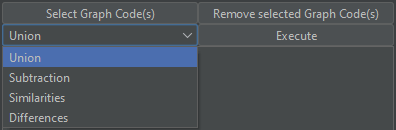
\includegraphics[width=9cm]{chapter/chapter_4/wireframe-impl-ui-4}
  \caption{Aus der Implementierung resultierende Schnittstelle zum Auswählen und Ausführen von Aktionen.}
  \label{sec4:impl:par:ui-elements:fig:wireframe-ui-4}
\end{figure}

Im Folgenden wird in \cref{sec4:impl:par:ui-elements:lst:editor-graph-code-p3}, dem dritten Teil der EditorGraphCode-Klasse, die Schnittstelle \circitem{5} bzw. Liste von Graph Codes genauer spezifiziert und im weiteren Verlauf erklärt.

\lstinputlisting[style=java-code, caption={EditorGraphCode-Klasse (Dritter Teil)}, label={sec4:impl:par:ui-elements:lst:editor-graph-code-p3}, firstnumber=52]{chapter/chapter_4/java/egc/EditorGraphCode-P3.java}

Zuerst werden Eigenschaften der Liste konfiguriert.
Eine dieser Eigenschaften ist z.B. der Auswahlmodus \textit{MULTIPLE\_INTERVAL\_SELECTION}, um eine mehrfache Auswahl in der Liste zu ermöglichen.

Die Liste ist mit dem Anwendungsfall \hyperref[sec3:model:uc-1.3]{UC-1.3} \enquote{Graph Code(s) auswählen} verbunden.
In Bezug auf den Anwendungsfall wird die Interaktion mit der Liste durch das Steuerelement \textit{GraphCodeSelectionListener} gesteuert, welches in einem Mechanismus (siehe \cref{sec3:model:par:mechanism-use-cases:fig:mech-uc-1.3}) identifiziert werden konnte.
Das Steuerelement \textit{GraphCodeSelectionListener} wird in \cref{sec4:impl:par:ui-elements:lst:select-gcs} genauer behandelt.
Zusätzlich besitzt die Liste weitere Steuerelemente, wie \textit{GraphCodeListMouseAdapter} und \textit{ListItemTransferHandler}, die ebenfalls in \cref{sec4:impl:par:ui-interaction} genauer behandelt werden.
Des Weiteren konnte in diesem Mechanismus, wie bereits auch schon in den vorherigen Mechanismen, die Komponente \textit{GraphCodeListElement} identifiziert werden.
Diese Komponente ist in Bezug auf die Liste von besonderer Bedeutung, da diese ein Element bzw. Eintrag in der Liste darstellt.
Der Quellcode für diese Komponente kann in \cref{sec4:impl:par:ui-elements:lst:gcle} eingesehen werden.

\clearpage

\lstinputlisting[style=java-code, caption={GraphCodeListElement-Klasse}, label={sec4:impl:par:ui-elements:lst:gcle}, firstnumber=1]{chapter/chapter_4/java/gcle/GraphCodeListElement.java}

\cref{sec4:impl:par:ui-elements:fig:wireframe-ui-5} zeigt ein Beispiel für die aus der Implementierung resultierende Liste mitsamt beispielhaften Einträgen für Graph Codes.

\begin{figure}[!ht]
  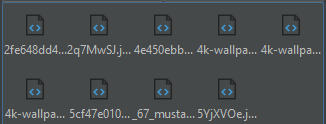
\includegraphics[width=9cm]{chapter/chapter_4/wireframe-impl-ui-5}
  \caption{Aus der Implementierung resultierende Liste mit beispielhaften Einträgen für Graph Codes.}
  \label{sec4:impl:par:ui-elements:fig:wireframe-ui-5}
\end{figure}

Schlussendlich wird in \cref{sec4:impl:par:ui-elements:lst:gct} die letzte Schnittstelle \circitem{6} \textit{GraphCodeTable} des Grundbereichs \textit{EditorGraphCode} behandelt und im weiteren Verlauf erklärt.

\lstinputlisting[style=java-code, caption={GraphCodeTable-Klasse}, label={sec4:impl:par:ui-elements:lst:gct}, firstnumber=1]{chapter/chapter_4/java/gct/GraphCodeTable.java}

Die Schnittstelle \textit{GraphCodeTable} besitzt zwei Elemente: Eine Tabelle zur Darstellung eines ausgewählten Graph Codes, umgesetzt durch ein \textit{JTable} und ein Platzhalter, zum Signalisieren, dass zu diesem Zeitpunkt noch kein Graph Code ausgewählt ist / wurde.
Die Tabelle wird in einem \textit{JScrollPane} eingebettet, um auch größere Tabellen darstellen zu können.
Des Weiteren ist ein wichtiger Teil dieser Klasse ein Datenmodell für die Tabelle, dargestellt durch die Komponente \textit{GraphCodeTableModel}.
Dieses Datenmodell wird der Tabelle zugewiesen und hat zur Aufgabe, die Informationen in einem Graph Code auf die Zeilen und Spalten der Tabelle abzubilden, sodass diese in Tabellenform dargestellt werden können.
Die wichtigste Methode der Klasse \textit{GraphCodeTable} ist \textit{setGraphCode}.
Diese Methode nimmt als Parameter einen ausgewählten Graph Code.
Anhand dieses Graph Codes werden Veränderungen an der Schnittstelle, sowie dem Datenmodell vorgenommen.
Sofern kein Graph Code ausgewählt ist, wird ein Platzhalter angezeigt.
Andernfalls wird dem Datenmodell der Graph Code zur Verarbeitung zugewiesen.

\cref{sec4:impl:par:ui-elements:fig:wireframe-ui-6} zeigt ein Beispiel für die aus der Implementierung resultierende Tabelle zur Darstellung eines ausgewählten Graph Codes.

\begin{figure}[!ht]
  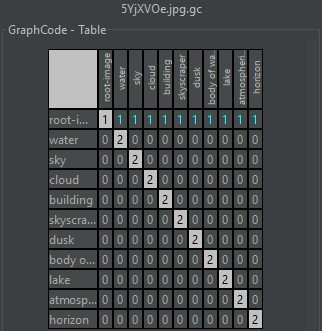
\includegraphics[width=8cm, keepaspectratio]{chapter/chapter_4/wireframe-impl-ui-6}
  \caption{Aus der Implementierung resultierende Tabelle zur Darstellung eines ausgewählten Graph Codes.}
  \label{sec4:impl:par:ui-elements:fig:wireframe-ui-6}
\end{figure}

Im Folgenden wird in \cref{sec4:impl:par:ui-elements:lst:editor-graph-code-p4}, der vierte und letzte Teil der EditorGraphCode-Klasse, genauer spezifiziert und im weiteren Verlauf erklärt.

\lstinputlisting[style=java-code, caption={EditorGraphCode-Klasse (Letzter Teil)}, label={sec4:impl:par:ui-elements:lst:editor-graph-code-p4}, firstnumber=58]{chapter/chapter_4/java/egc/EditorGraphCode-P4.java}

\cref{sec4:impl:par:ui-elements:lst:editor-graph-code-p4} zeigt das abschließende Zusammenfügen der Schnittstellen \circitem{4}, \circitem{5} und \circitem{6}.
Zusammengefügt ergeben diese Schnittstellen den Grundbereich \textit{EditorGraphCode}.
Damit ist der Grundbereich \circitem{1}, \textit{EditorGraphCode}, abgeschlossen.
\cref{sec4:impl:par:ui-elements:fig:wireframe-ui-left-complete} zeigt abschließend die vollständige Benutzeroberfläche des aus der Implementierung resultierenden Grundbereichs \textit{EditorGraphCode} mitsamt Beispielen.

\begin{figure}[!ht]
  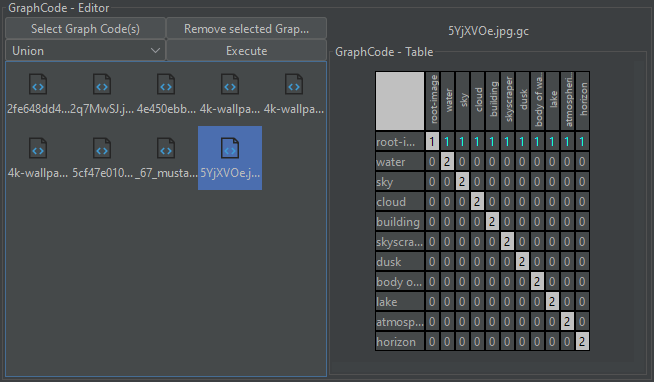
\includegraphics[width=\textwidth]{chapter/chapter_4/wireframe-impl-ui-left-complete}
  \caption{Vollständige Oberfläche des aus der Implementierung resultierenden Grundbereichs \textit{EditorGraphCode}.}
  \label{sec4:impl:par:ui-elements:fig:wireframe-ui-left-complete}
\end{figure}

Im weiteren Verlauf dieses Abschnitts wird in \cref{sec4:impl:par:ui-elements:lst:explanation-panel} der Grundbereich \circitem{2}, \textit{ExplanationPanel}, behandelt und die darin enthaltenen Schnittstellen detailliert erläutert.

\clearpage

\begin{figure}[!ht]
  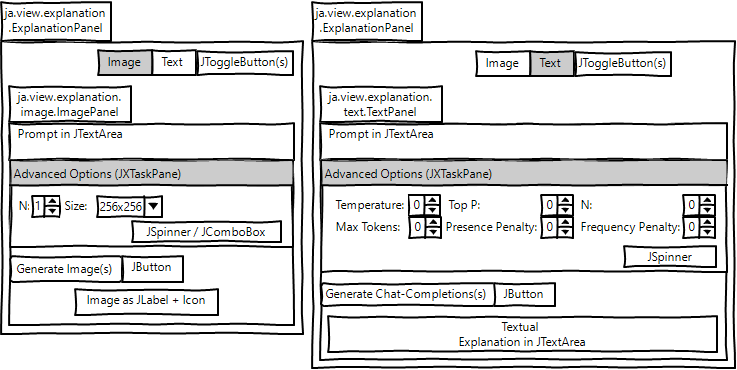
\includegraphics[width=\textwidth]{chapter/chapter_4/wireframe-impl-right}
  \caption{Grundbereich \textit{ExplanationPanel} zur Generierung von visuellen Erklärungen (links) und textuellen Erklärungen (rechts).}
  \label{sec4:impl:subsubsec:ui:fig:wireframe-explanation-panel}
\end{figure}

\cref{sec4:impl:subsubsec:ui:fig:wireframe-explanation-panel} zeigt den nächsten Grundbereich \circitem{2}, \textit{ExplanationPanel}, umgesetzt durch die Klasse \textit{ja.view.explanation.ExplanationPanel}, in welchem Benutzer durch geeignete Interaktionsmöglichkeiten die Generierung von textuellen und visuellen Erklärungen zu Graph Codes durchführen können.
Hierzu besitzt der Grundbereich \textit{ExplanationPanel} eine Fläche, in der Komponenten miteinander ausgewechselt werden können.
Genauer wird zwischen den zwei Komponenten: \textit{TextPanel} und \textit{ImagePanel}, gewechselt.

\lstinputlisting[style=java-code, caption={ExplanationPanel-Klasse}, label={sec4:impl:par:ui-elements:lst:explanation-panel}, firstnumber=1]{chapter/chapter_4/java/exp/ExplanationPanel.java}

Der Grundbereich \textit{ExplanationPanel} besitzt zwei Knöpfe (\textit{JToggleButton}) \enquote{Image} und \enquote{Text}, mit welchen zwischen den Schnittstellen \textit{ImagePanel}, zum Generieren von visuellen Erklärungen zu Graph Codes und \textit{TextPanel}, zum Generieren von textuellen Erklärungen zu Graph Codes, hin- und hergeschaltet werden kann.
Die Interaktion für diese Knöpfe wird innerhalb der Klasse durch die Methode \textit{actionPerformed} umgesetzt.
Hierfür implementiert die Klasse das Interface \textit{ActionListener} und wird den Knöpfen registriert.
Damit nur ein Knopf zeitgleich aktiviert sein kann, werden die Knöpfe einer \textit{ButtonGroup} hinzugefügt.
Die zwei Schnittstellen \textit{TextPanel} und \textit{ImagePanel} werden beide initialisiert und existieren zum selben Zeitpunkt.
Jedoch kann, in Abhängigkeit des gewählten Knopfes, immer nur eine Schnittstelle angezeigt werden.
Am Anfang ist die Schnittstelle \textit{ImagePanel} zu sehen.

Des Weiteren umfasst die Klasse zwei Methoden: \textit{setGraphCode} und \textit{actionPerformed}.
Die Methode \textit{setGraphCode} delegiert einen Graph Code an die Schnittstellen \textit{ImagePanel} und \textit{TextPanel}, wo diese dann entsprechend weiter verarbeitet werden.
Die Methode \textit{actionPerformed} wird durch das Interface \textit{ActionListener} bereitgestellt und durch die Methode \textit{addActionListener} auf die Knöpfe registriert.
Diese Methode übernimmt das Hin- und Herschalten zwischen \textit{Text}- oder \textit{ImagePanel} und entfernt \textit{TextPanel}, sofern \textit{ImagePanel} ausgewählt wird und vice versa.

Im Folgenden werden die Schnittstellen \textit{TextPanel} und \textit{ImagePanel} genauer erklärt.
Dabei wird zuerst \textit{TextPanel} und dann \textit{ImagePanel} behandelt.
Grund für diese Reihenfolge ist die Art wie die Erklärungen, ob textuell oder visuell, generiert werden.
Wie bereits in \cref{sec3:model:subsubsec:genai-integration} konzipiert wurde, wird beim Erzeugen einer visuellen Erklärung erst eine mit Tokenbegrenzung versehene, textuelle Erklärung generiert, die eine visuelle Beschreibung darstellen und als Grundlage für eine Bilderzeugung dienen soll.
Somit ist das Generieren einer textuellen Erklärung ein wichtiger Zwischenschritt in der Generierung einer visuellen Erklärung und wird als thematisiert.

\lstinputlisting[style=java-code, caption={TextPanel-Klasse}, label={sec4:impl:par:ui-elements:lst:text-panel-p1}, firstnumber=1]{chapter/chapter_4/java/exp/text/TextPanel-P1.java}

\cref{sec4:impl:par:ui-elements:lst:text-panel-p1} zeigt den ersten Teil der Klasse \textit{TextPanel} und die ersten oberen Schnittstellen \circitem{8} und \circitem{9}.
Genauer sind dies ein Textfeld für die Prompt, eingeführt durch die Variable \textit{promptArea} und eine ein- und ausklappbare Fläche für erweiterte Optionen, eingeführt durch die Variable \textit{advancedOptions}.
Diese ein- und ausklappbare Fläche wird durch die Klasse \textit{JXTaskPane} umgesetzt und ist Teil der Abhängigkeit \textit{SwingX}. % Referenz
Dieser Fläche werden wiederum mehrere Elemente in Form von \textit{JLabels} und \textit{JSpinner} hinzugefügt, die die erweiterten Optionen darstellen.
Mithilfe der erweiterten Optionen können Anfragen an den Endpunkt Text angepasst werden und die Wahrscheinlichkeiten für bestimmte Ausgaben beeinflusst werden.
Da diese Optionen für gewöhnlich eingeschränkte Wertebereiche aufweisen, werden den \textit{JSpinner} daher Datenmodelle (\textit{SpinnerNumberModel}) zugewiesen, um Benutzereingaben einzuschränken.
\cref{sec4:impl:par:ui-elements:fig:wireframe-ui-8+9} zeigt die ersten beiden oberen Schnittstellen \circitem{8} und \circitem{9} für \textit{TextPanel}.

\begin{figure}[!ht]
  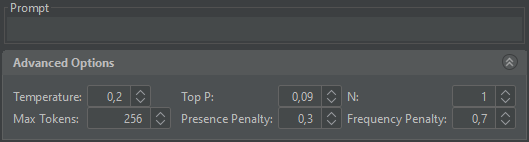
\includegraphics[width=0.9\textwidth]{chapter/chapter_4/wireframe-impl-ui-8+9}
  \caption{Textfeld für die Prompt und erweiterte Optionen.}
  \label{sec4:impl:par:ui-elements:fig:wireframe-ui-8+9}
\end{figure}

\lstinputlisting[style=java-code, caption={TextPanel-Klasse (Zweiter Teil)}, label={sec4:impl:par:ui-elements:lst:text-panel-p2}, firstnumber=35]{chapter/chapter_4/java/exp/text/TextPanel-P2.java}

\cref{sec4:impl:par:ui-elements:lst:text-panel-p2} zeigt den zweiten Teil der Klasse \textit{TextPanel} und die untere Schnittstelle \circitem{10}.
Dies ist im Fall der Klasse \textit{TextPanel} ein Textfeld für die generierte textuelle Erklärung und diese wird im Quellcode als Variable \textit{textResponseArea} eingeführt.
Zusätzlich wird ein Knopf \enquote{Generate Chat-Completion(s)} hinzugefügt und die Klasse als \textit{ActionListener} dem Knopf registriert.
Hierfür implementiert die Klasse \textit{TextPanel} das Interface \textit{ActionListener}.
Aufgabe des Knopfes ist das Erstellen und Verarbeiten einer Anfrage an den Endpunkt Text der OpenAI-Schnittstelle.
\cref{sec4:impl:par:ui-elements:fig:wireframe-text-complete} zeigt die vollständige Schnittstelle für die Klasse \textit{TextPanel}.

\begin{figure}[!ht]
  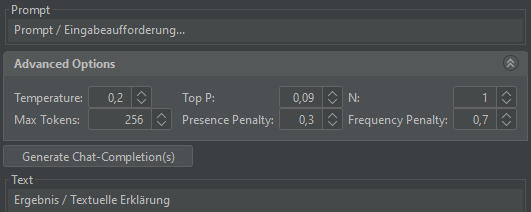
\includegraphics[width=0.9\textwidth]{chapter/chapter_4/wireframe-impl-text-complete}
  \caption{Vollständige Schnittstelle für die Klasse \textit{TextPanel}.}
  \label{sec4:impl:par:ui-elements:fig:wireframe-text-complete}
\end{figure}

\lstinputlisting[style=java-code, caption={TextPanel-Klasse (Letzter Teil)}, label={sec4:impl:par:ui-elements:lst:text-panel-p3}, firstnumber=49]{chapter/chapter_4/java/exp/text/TextPanel-P3.java}

\cref{sec4:impl:par:ui-elements:lst:text-panel-p3} zeigt den letzten Teil der Klasse \textit{TextPanel} und die für diese Klasse wichtigen Methoden \textit{setGraphCode}, \textit{setUpPrompt} und \textit{actionPerformed}.
Die Methode \textit{setGraphCode} hat die Verarbeitung eines Graph Codes zur Aufgabe und ruft hierfür wiederum die Methode \textit{setUpPrompt} auf.
Diese Methode ruft die Informationen in einem Graph Code ab und erstellt aus diesen eine Reihe an Textnachrichten, die zusammen eine Prompt darstellen.
Das Ergebnis dieses Aufrufs wird dann in einem dafür vorgesehenen Textfeld angezeigt.
In dieser Methode wird somit die Transformation von Graph Codes vorgenommen.
Die genauen Details der Implementierung dieser Methode werden daher in \cref{sec4:impl:subsubsec:gc-transformation} behandelt.
Schlussendlich hat die Methode \textit{actionPerformed} die Erzeugung einer Erklärung und der damit verbundenen Erzeugung einer Anfrage an den Endpunkt Text zur Aufgabe.
In dieser Methode wird somit die Integration des Endpunkts Text vorgenommen.
Genauere Details dieser Methode zum Erstellen einer Anfrage an den Endpunkt Text werden in \cref{sec4:impl:subsubsec:endpoint-integration} behandelt.

Im Folgenden zeigt \cref{sec4:impl:par:ui-elements:lst:image-panel} die Schnittstelle \textit{ImagePanel}.
\cref{sec4:impl:par:ui-elements:lst:image-panel} verhält sich dabei analog zu den \cref{sec4:impl:par:ui-elements:lst:text-panel-p1,sec4:impl:par:ui-elements:lst:text-panel-p2,sec4:impl:par:ui-elements:lst:text-panel-p3}.
Als solches ist die Schnittstelle \textit{ImagePanel} im Aufbau seiner Benutzeroberfläche, mit Außnahme der erweiterten Optionen und dem \textit{JLabel} + Icon zum Darstellen eines erzeugten Bildes im Vergleich zum Textfeld, identisch (siehe \cref{sec4:impl:subsubsec:ui:fig:wireframe-explanation-panel}).
Ein weiterer Unterschied besteht in der Methode \textit{actionPerformed} beim Generieren einer visuellen Erklärung zu einem Graph Code.
Hier wird zuerst eine spezielle, textuelle Erklärung generiert, die dann wiederum als Eingabe für den Endpunkt Bild zum Generieren einer visuellen Erklärung genutzt wird.
Genauere Details zum Erstellen einer Anfrage an den Endpunkt Bild werden in \cref{sec4:impl:subsubsec:endpoint-integration} behandelt.

\lstinputlisting[style=java-code, caption={ImagePanel-Klasse}, label={sec4:impl:par:ui-elements:lst:image-panel}, firstnumber=1]{chapter/chapter_4/java/exp/img/ImagePanel.java}

Damit sind beide Schnittstellen \textit{TextPanel} und \textit{ImagePanel} abschließend beschrieben und erklärt.
\cref{sec4:impl:par:ui-elements:fig:wireframe-image-complete} zeigt die vollständige Schnittstelle für die Klasse \textit{ImagePanel}.
Der Grundbereich \circitem{2}, \textit{ExplanationPanel}, ist damit abgeschlossen.

\begin{figure}[!ht]
  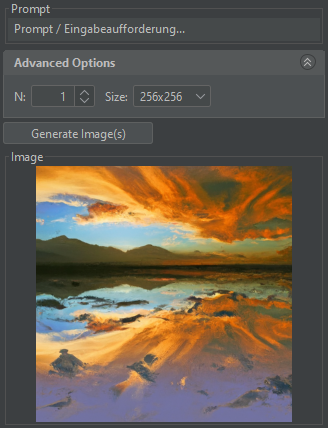
\includegraphics{chapter/chapter_4/wireframe-impl-image-complete}
  \caption{Vollständige Schnittstelle für die Klasse \textit{ImagePanel}.}
  \label{sec4:impl:par:ui-elements:fig:wireframe-image-complete}
\end{figure}

\FloatBarrier

Im weiteren Verlauf dieses Abschnitts wird in \cref{sec4:impl:par:ui-elements:lst:explainer-console} schlussendlich die Implementierung des letzten Grundbereichs \circitem{3}, \textit{ExplainerConsole}, behandelt und erklärt.
Die allgemeine Aufgabe des Grundbereichs \textit{ExplainerConsole} ist es wichtige Informationen über Prozesse des Programms zu loggen.
Wichtige Informationen können Bestätigungen von Aktionen und Fehlermeldungen umfassen.

\lstinputlisting[style=java-code, caption={ExplainerConsole-Klasse}, label={sec4:impl:par:ui-elements:lst:explainer-console}, firstnumber=1]{chapter/chapter_4/java/exc/ExplainerConsole.java}

Die Benutzeroberfläche des dritten Grundbereichs, \textit{ExplainerConsole}, besteht aus zwei nennenswerten Komponenten: Einem Textfeld für die angegebenen Informationen, sowie eine Toolbar mit Button zum Leeren des Textfeldes.
Das Textfeld ist eine Instanz der Klasse \textit{RSyntaxTextArea} und entstammt der gleichnamigen Abhängigkeit.
Die beiden Methoden \textit{onInsert} und \textit{onClear} sind Teil des eigens entwickelten Interfaces \textit{ITextInsertListener} und behandeln das Einfügen von Text in die Konsole, sowie das Leeren des Textfeldes der Konsole.

Damit sind alle Grundbereiche der Benutzeroberfläche des Programms abgeschlossen.
Der Zusammenschluss dieser Grundbereiche wird, wie bereits am Anfang des Abschnitts angemerkt, durch die Methode \textit{initComponents} in der Klasse \textit{ExplainerFrame} vorgenommen (siehe \cref{sec4:impl:par:ui-elements:lst:explainer-frame}).
Die genaue Implementierung dieser Methode kann in \cref{sec4:impl:par:ui-elements:lst:initComps} eingesehen werden und verdeutlicht den Zusammenschluss bzw. das Zusammenfügen der einzelnen Grundbereiche in das Fundament der gesamten Benutzungsschnittstelle.

\lstinputlisting[style=java-code, caption={Zusammenschluss der Grundbereiche}, label={sec4:impl:par:ui-elements:lst:initComps}, firstnumber=1]{chapter/chapter_4/java/methods/initComponents.java}

Besonders erwähnenswert für diese Methode ist die Komponente \textit{JXMultiSplitPane}, die Teil der Abhängigkeit \textit{SwingX} ist.
Zu dieser gehören ebenfalls die Komponenten \textit{MultiSplitLayout}, \textit{Split}, \textit{Divider} und \textit{Leaf}, die den Aufbau beschreiben.
Mithilfe der Komponente \textit{JXMultiSplitPane} können auf einfache Art und Weise und ohne großen Aufwand Schnittstellen angelegt werden, die in ihrer Größe anpassbar sind und die andernfalls nur durch aufwendige Verschachtelung mehrerer \textit{JSplitPane}'s erzeugt werden könnten.

In diesem Abschnitt wurde die Implementierung der Benutzeroberfläche beschrieben.
Hierfür wurden die Quellcodes für die in der Benutzeroberfläche verbauten Komponenten kompakt dargestellt und detailliert erläutert.
Eine abschließende Gesamtabbildung der vollständigen Benutzeroberfläche samt Beispielen kann im \cref{sec4:impl:subsec:summary} \enquote{Zusammenfassung} in den \cref{sec4:impl:subsubsec:summary-findings:fig:ui-ex-1,sec4:impl:subsubsec:summary-findings:fig:ui-ex-2,sec4:impl:subsubsec:summary-findings:fig:ui-ex-3} eingesehen werden.
Im folgenden Abschnitt wird die Interaktion mit und zwischen den in diesem Abschnitt beschriebenen Komponenten der Benutzeroberfläche thematisiert.

\FloatBarrier

\paragraph{Interaktion mit der Benutzeroberfläche}
\label{sec4:impl:par:ui-interaction}
In diesem Abschnitt wird die Implementierung der Interaktion zwischen Benutzern und Komponenten der Benutzeroberfläche genauer beschrieben.
Darüber hinaus werden auch die Zusammenhänge zwischen den Komponenten genauer betrachtet.
Dies umfasst Beschreibungen, wie die Komponenten gegenseitig miteinander interagieren und sich untereinander beeinflussen.
Die Beschreibung der Interaktion konzentriert sich dabei im Wesentlichen auf die Anwendungsfälle \hyperref[sec3:model:uc-1.1]{UC-1.1}, \hyperref[sec3:model:uc-1.2]{UC-1.2}, \hyperref[sec3:model:uc-1.3]{UC-1.3} und \hyperref[sec3:model:uc-1.5]{UC-1.5}.
Dies sind die Anwendungsfälle, in welchen Benutzer durch die Interaktion mit Komponenten in der Benutzeroberfläche komplexe und bedeutende Abläufe in Bezug auf Graph Codes in Gang setzen, die wiederum Einfluss auf andere Komponenten haben.
Allerdings sind von diesen Beschreibungen die verbleibenden Anwendungsfälle: \hyperref[sec3:model:uc-1.4]{UC-1.4} \enquote{Operation auswählen}, \hyperref[sec3:model:uc-1.7]{UC-1.7} \enquote{Erweiterte Optionen anpassen} (Interaktionen werden bereits durch jeweilige Komponenten bereitgestellt), \hyperref[sec3:model:uc-1.6]{UC-1.6} \enquote{Erklärungstyp umschalten} (Interaktion beeinflusst zwar die Komponente \textit{ExplanationPanel}, umfasst im Wesentlichen aber nur das Entfernen und Hinzufügen von \textit{ImagePanel} und \textit{TextPanel}) ausgenommen.
Der verbleibende Anwendungsfall \hyperref[sec3:model:uc-1.8]{UC-1.8} wird explizit in \cref{sec4:impl:subsubsec:endpoint-integration} behandelt.

\cref{sec4:impl:par:ui-interaction:lst:import-gcs} zeigt das Steuerelement \textit{ImportGraphCodesController}, welches mit dem Anwendungsfall \hyperref[sec3:model:uc-1.1]{UC-1.1} \enquote{Graph Code(s) importieren} assoziiert ist.
Das Steuerelement wird durch einen Klick auf den Knopf \enquote{Import Graph Code(s)} initiiert und importiert ein oder mehrere aus einem Auswahldialog ausgewählte Graph Code Dateien in die Liste für Graph Codes (siehe \cref{sec3:model:par:wireframe:fig:stage-2+3} \circitem{5}).

\lstinputlisting[style=java-code, caption={ImportGraphCodesController-Klasse}, label={sec4:impl:par:ui-interaction:lst:import-gcs}, firstnumber=1]{chapter/chapter_4/java/interaction/ImportGraphCodesController.java}

Der Auswahldialog wird, wie auch bereits in \cref{sec3:model:par:mechanism-use-cases:fig:mech-uc-1.1} identifiziert, durch die Komponente \textit{JFileChooser} bereitgestellt.
Durch eine Anpassung des Verzeichnisses zeigt der Dialog relativ auf das Verzeichnis des Projekts, in welchem Graph Code Dateien gespeichert sind.
Weitere Anpassungen des Dialogs umfassen einen Dateifilter, sodass Benutzern nur Dateien mit der Endung \enquote{.gc} angezeigt werden bzw. nur diese ausgewählt werden können, sowie eine mögliche Mehrfachauswahl von Dateien.
Werden die ausgewählten Dateien geöffnet, so werden für alle ausgewählten Dateien Einträge (\textit{GraphCodeListElement}) für die Liste geschaffen, die dann dem Datenmodell (\textit{DefaultListModel}) der Liste hinzugefügt werden.

Damit entspricht der Ablauf der Aktionen in \cref{sec4:impl:par:ui-interaction:lst:import-gcs} grundsätzlich den modellierten Abläufen im UML-Sequenzdiagramm, dargestellt in \cref{sec3:model:par:seq-use-cases:fig:seq-diag-uc-1.1}, für den Anwendungsfall \hyperref[sec3:model:uc-1.1]{UC-1.1}.

% Steuerelement: Durch welche Interaktion wird diese Aktion iniiert? -> Benutzer muss auf Knopf ... klicken.
% Dann beschreiben, wie der Ablauf der Aktionen aussieht... und diese mit der Modellierung vergleichen?
% Hier auf die notwendigen Komponenten dieser Aktionen

% Schritt für Schritt dann den Ablauf der Aktionen beschreiben...
% Für jede Aktionen betrachten, ob es sinnvoll oder notwendig ist auf die an dieser Aktion beteiligten Komponenten einzugehen...
% Wenn ja, dann auf jeweilige Komponenten verweisen und auch auf die Identifizierung dieser Komponenten in Mechanismen verweisen...
% Später dann den Ablauf der Aktionen mit dem in der Modellierung entsprechendem Sequenzdiagramm "vergleichen"...

\cref{sec4:impl:par:ui-elements:lst:remove-gcs} zeigt das Steuerelement \textit{RemoveSelectedGraphCodesController}, welches mit dem Anwendungsfall \hyperref[sec3:model:uc-1.2]{UC-1.2} \enquote{Graph Code(s) entfernen} assoziiert ist.
Das Steuerelement wird durch einen Klick auf den Knopf \enquote{Remove selected Graph Code(s)} initiiert und entfernt die in der Liste ausgewählten Graph Codes.

\lstinputlisting[style=java-code, caption={RemoveSelectedGraphCodesController-Klasse}, label={sec4:impl:par:ui-elements:lst:remove-gcs}, firstnumber=1]{chapter/chapter_4/java/interaction/RemoveSelectedGraphCodesController.java}

Voraussetzung für das erfolgreiche Entfernen von ein oder mehreren Graph Code Datei(en) ist, dass die Liste einen oder mehrere Graph Code(s) enthält bzw. diese von einem Benutzer ausgewählt worden sind.
Hierfür wird die Liste und das Datenmodell der Liste benötigt.
In einem ersten Schritt werden die Indizes von potentiell ausgewählten Einträgen der Liste abgefragt und geprüft, ob die Anzahl der ausgewählten Einträge größer null ist.
Sofern dies der Fall ist, werden diese Indizes durchlaufen und dem Datenmodell mitgeteilt, dass der Eintrag am entsprechenden Index entfernt werden soll.

Damit entspricht der Ablauf der Aktionen in \cref{sec4:impl:par:ui-elements:lst:remove-gcs} ebenfalls grundsätzlich den modellierten Abläufen im UML-Sequenzdiagramm, dargestellt in \cref{sec3:model:par:seq-use-cases:fig:seq-diag-uc-1.2}, für den Anwendungsfall \hyperref[sec3:model:uc-1.2]{UC-1.2}.

\cref{sec4:impl:par:ui-elements:lst:select-gcs} zeigt das Steuerelement \textit{GraphCodeSelectionListener}, welches mit dem Anwendungsfall \hyperref[sec3:model:uc-1.3]{UC-1.3} \enquote{Graph Code(s) auswählen} assoziiert ist.
Das Steuerelement wird durch die Auswahl eines oder mehrerer Elemente in der Liste initiiert und beeinflusst daraufhin durch Initiierung weiterer Aktionen andere Benutzungsschnittstellen, indem Informationen an diese weitergegeben werden.

\lstinputlisting[style=java-code, caption={GraphCodeSelectionListener-Klasse}, label={sec4:impl:par:ui-elements:lst:select-gcs}, firstnumber=1]{chapter/chapter_4/java/interaction/GraphCodeSelectionListener.java}

Voraussetzung für das erfolgreiche Auswählen von ein oder mehreren Graph Code Datei(en) ist, dass die Liste einen oder mehrere Graph Code(s) enthält.
Ist ein Eintrag aus der Liste ausgewählt, so können andere Benutzungsschnittstellen über die Informationen in diesem Eintrag informiert und angepasst werden.
Die Informationen eines Eintrages umfassen den aus der Datei gelesenen Graph Code und den Dateinamen.
Zu den angepassten Benutzungsschnittstellen gehören somit die Tabelle zur Darstellung des Graph Codes \textit{GraphCodeTable} inklusive eines Textfeldes zur Anzeige des Dateinamens, sowie die Schnittstelle \textit{ExplanationPanel} zur Erzeugung von Erklärungen.
Die Informationen eines ausgewählten Eintrages werden hierbei jeweils an \textit{GraphCodeTable} und \textit{ExplanationPanel} delegiert, woraufhin diese in den entsprechenden Komponenten weiterverarbeitet werden.

Damit entspricht der Ablauf der Aktionen in \cref{sec4:impl:par:ui-elements:lst:select-gcs} ebenfalls grundsätzlich den modellierten Abläufen im UML-Sequenzdiagramm, dargestellt in \cref{sec3:model:par:seq-use-cases:fig:seq-diag-uc-1.3}, für den Anwendungsfall \hyperref[sec3:model:uc-1.3]{UC-1.3}.

\cref{sec4:impl:par:ui-elements:lst:mouse-gcs} zeigt das Steuerelement \textit{GraphCodeListMouseAdapter}.
Dieses Steuerelement ist nicht explizit mit einem Anwendungsfall assoziiert und wird durch eine Interaktion der Maus mit der Liste initiiert.
Ist diese Interaktion ein Doppelklick, so wird in der Liste geprüft, ob an der Position der Interaktion ein Eintrag vorliegt.
Sofern dies der Fall ist, wird der Index dieses Eintrags bestimmt und der Eintrag aus dem Datenmodell \textit{DefaultListModel} extrahiert.
Dem Benutzer wird dann ein Dialog angezeigt, mit welchem dieser eine Umbenennung des Eintrags vornehmen kann.

\lstinputlisting[style=java-code, caption={GraphCodeListMouseAdapter-Klasse}, label={sec4:impl:par:ui-elements:lst:mouse-gcs}, firstnumber=1]{chapter/chapter_4/java/interaction/GraphCodeListMouseAdapter.java}

Neben dem Steuerelement \textit{GraphCodeListMouseAdapter} wird der Liste noch ein weiteres Steuerelement hinzugefügt bzw. registriert.
Dieses Steuerelement heißt \textit{ListItemTransferHandler} und ermöglicht das Verschieben von Einträgen mittels Drag und Drop.
% Der Quellcode für diese und weitere Komponenten kann in ... eingesehen werden.

\cref{sec4:impl:par:ui-elements:lst:calculate-gcs-p1,sec4:impl:par:ui-elements:lst:calculate-gcs-p2,sec4:impl:par:ui-elements:lst:calculate-gcs-p3,sec4:impl:par:ui-elements:lst:calculate-gcs-p4,sec4:impl:par:ui-elements:lst:calculate-gcs-p5} zeigen das Steuerelement \textit{GraphCodeCalculationController}, welches mit dem Anwendungsfall \hyperref[sec3:model:uc-1.5]{UC-1.5} \enquote{Operation ausführen} assoziiert ist.
Das Steuerelement wird durch einen Klick auf den Knopf \textit{Execute} initiiert und führt die in Anwendungsfall \hyperref[sec3:model:uc-1.4]{UC-1.4} ausgewählte Operation auf den ausgewählten Graph Codes aus.

\cref{sec4:impl:par:ui-elements:lst:calculate-gcs-p1} zeigt die für die Anwendung von Operationen auf Graph Codes notwendigen Komponenten.
Dies umfasst die in Anwendungsfall \hyperref[sec3:model:uc-1.4]{UC-1.4} ausgewählte Operation \textit{actionItem}, die in den folgenden \cref{sec4:impl:par:ui-elements:lst:calculate-gcs-p2,sec4:impl:par:ui-elements:lst:calculate-gcs-p3,sec4:impl:par:ui-elements:lst:calculate-gcs-p4,sec4:impl:par:ui-elements:lst:calculate-gcs-p5} in einem Switch-Statement zur Differenzierung der auszuführenden Aktionen dienen wird, sowie eine Liste \textit{selGraphCodes} der ausgewählten Einträge aus der Liste.

\lstinputlisting[style=java-code, caption={GraphCodeCalculationController-Klasse}, label={sec4:impl:par:ui-elements:lst:calculate-gcs-p1}, firstnumber=1]{chapter/chapter_4/java/interaction/GraphCodeCalculationController-P1.java}

\cref{sec4:impl:par:ui-elements:lst:calculate-gcs-p2} zeigt die Anwendung der Operation \enquote{Union}.
Die Operation zur Berechnung der Vereinigung von Graph Codes wird bereits vom GMAF durch die Komponente \textit{GraphCodeCollection} bereitgestellt.
Um diese Operation nutzen zu können, muss in einem ersten Schritt aus der Liste an Einträgen eine Liste an Graph Codes geschaffen werden.
Dies wird durch das Abbilden eines Eintrages auf einen Graph Code erreicht.
Weiter wird die Liste in einen Vektor umgewandelt, da die Funktion der Vereinigung einen Vektor als Eingabe erwartet.
Die Ausgabe der Vereinigung ist wiederum ein Graph Code, welcher dann in einen neu erstellten Eintrag eingebettet wird.
Über einen Dialog kann dann ein Benutzer nach Anwendung der Operation dem Eintrag einen neuen Namen zuweisen.
Der Eintrag wird dann dem Datenmodell der Liste hinzugefügt.

\lstinputlisting[style=java-code, caption={GraphCodeCalculationController-Klasse}, label={sec4:impl:par:ui-elements:lst:calculate-gcs-p2}, firstnumber=1]{chapter/chapter_4/java/interaction/GraphCodeCalculationController-P2.java}

\cref{sec4:impl:par:ui-elements:lst:calculate-gcs-p3} zeigt die Anwendung der Operation \enquote{Subtraction}.
Auch die Operation zur Berechnung der Subtraktion eines Graph Codes von einem anderen Graph Code wird durch die Komponente \textit{GraphCodeCollection} bereitgestellt.
Im Fall dieser Operation wird aus den ausgewählten Eintrag allerdings nur der erste und zweite Eintrag berücksichtigt.
Ausgabe der Operation der Subtraktion ist ebenfalls ein Graph Code.
Die verbleibenden Aktionen verhalten sich analog zur Operation der Vereinigung von Graph Codes.

\clearpage

\lstinputlisting[style=java-code, caption={GraphCodeCalculationController-Klasse}, label={sec4:impl:par:ui-elements:lst:calculate-gcs-p3}, firstnumber=1]{chapter/chapter_4/java/interaction/GraphCodeCalculationController-P3.java}

\cref{sec4:impl:par:ui-elements:lst:calculate-gcs-p4} zeigt die Anwendung der Operation \enquote{Similarities}.
Die Operation zur Berechnung der Gemeinsamkeiten von Graph Codes wurde bereits in \cref{sec3:model:par:mechanism-use-cases:alg:sim} als Teil der Modellierung in einem Pseudoalgorithmus vorgestellt.
Die Implementierung dieses Algorithmus ist in \cref{sec4:impl:par:ui-elements:lst:calculate-sim} einsehbar und wird ähnlich wie die Operationen zur Vereinigung und Subtraktion in die Klasse \textit{GraphCodeCollection} eingebunden.

\lstinputlisting[style=java-code, caption={GraphCodeCalculationController-Klasse}, label={sec4:impl:par:ui-elements:lst:calculate-gcs-p4}, firstnumber=1]{chapter/chapter_4/java/interaction/GraphCodeCalculationController-P4.java}

\lstinputlisting[style=java-code, caption={Algorithmus zur Bestimmung der Gemeinsamkeiten von Graph Codes}, label={sec4:impl:par:ui-elements:lst:calculate-sim}, firstnumber=1]{chapter/chapter_4/java/algorithm/Alg-Similarities.java}

Die für die Anwendung der Operation \enquote{Similarities} notwendigen Schritte sind äquivalent zu den Schritten der Operation der Vereinigung, mit Ausnahme des Aufrufs der spezifischen Funktion, deren Schritte im Weiteren genauer beschrieben werden.

In einem ersten Schritt wird in Zeile 5 die Vereinigung aller Graph Codes berechnet.
Ergebnis ist ein Graph Code mit einem Wörterbuch, welches alle Merkmale aller Graph Codes enthält.
In einem weiteren Schritt werden von Zeile 11 bis 13 alle Graph Codes in einer Schleife durchlaufen.
Bei jedem Durchlauf werden alle Elemente aus dem Wörterbuch der Vereinigung entfernt, die nicht in irgendeinem Wörterbuch der anderen Graph Codes vorhanden sind.
Hierzu wird in Zeile 7 eine Kopie des Wörterbuchs erstellt und später verwendet.
Übrig bleiben alle Elemente, die auch in den Wörterbüchern aller anderen Graph Codes vorkommen.
Dieses Wörterbuch wird dann dem Ergebnis zugewiesen.
Von Zeile 18 bis 30 werden dann in einem letzten Schritt für alle Graph Codes alle Elemente zeilen- und spaltenweise durchlaufen, um die Werte für diese Einträge zu bestimmen und dem Ergebnis zuzuweisen.
Schlussendlich ist das Ergebnis dieser Funktion ein Graph Code, dessen Wörterbuch alle gemeinsamen Elemente bzw. Merkmale und Werte aller verarbeiteten Graph Codes enthält.
Auf die Modellierung rückblickend ist die Implementierung dieses Algorithmus somit sehr ähnlich zu dem konzipierten Pseudoalgorithmus.

\cref{sec4:impl:par:ui-elements:lst:calculate-gcs-p5} zeigt die Anwendung der Operation \enquote{Differences}.
Die Operation zur Berechnung der Unterschiede von Graph Codes wurde bereits in \cref{sec3:model:par:mechanism-use-cases:alg:dif} als Teil der Modellierung in einem Pseudoalgorithmus vorgestellt.
Die Implementierung dieses Algorithmus ist in \cref{sec4:impl:par:ui-elements:lst:calculate-diff} einsehbar und wird ebenfalls in die Klasse \textit{GraphCodeCollection} eingebunden.

\lstinputlisting[style=java-code, caption={GraphCodeCalculationController-Klasse}, label={sec4:impl:par:ui-elements:lst:calculate-gcs-p5}, firstnumber=1]{chapter/chapter_4/java/interaction/GraphCodeCalculationController-P5.java}

\lstinputlisting[style=java-code, caption={Algorithmus zur Bestimmung der Unterschiede von Graph Codes}, label={sec4:impl:par:ui-elements:lst:calculate-diff}, firstnumber=1]{chapter/chapter_4/java/algorithm/Alg-Differences.java}

Die für die Anwendung der Operation \enquote{Differences} notwendigen Schritte sind ebenfalls äquivalent zu den Schritten der Operation der Vereinigung, mit Ausnahme des Aufrufs der spezifischen Funktion.

Der in \cref{sec4:impl:par:ui-elements:lst:calculate-diff} dargestellte Algorithmus zur Berechnung der Unterschiede von Graph Codes ist dabei nahezu identisch mit dem in \cref{sec4:impl:par:ui-elements:lst:calculate-sim} dargestellten Algorithmus zur Berechnung der Gemeinsamkeiten.
Folglich ist die Implementierung dieses Algorithmus ebenfalls sehr ähnlich zu dem entsprechend konzipierten Pseudoalgorithmus.
Der bedeutende Unterschied besteht in der Art der Berechnung des Wörterbuchs.
Genauer ist die Differenz aller Graph Codes die Vereinigung aller Graph Codes abzüglich der Gemeinsamkeiten aller Graph Codes.
Die Berechnung dieser Differenz geschieht in Zeile 17 und nutzt hierfür die Abhängigkeit \textit{Guava} von Google.
Die Methode \textit{difference} erwartet als Eingabe zwei Sets.
Dies kann ein Problem darstellen, da ein Set nicht die Ordnung bzw. Reihenfolge seiner Elemente beibehält, diese aber für das Wörterbuch eines Graph Codes besonders wichtig ist.
Daher werden in diesem Fall die Wörterbücher in ein \textit{LinkedHashSet} übernommen, welche die Reihenfolge ihre Elemente beibehalten.
Diese werden dann als Eingabe für die Funktion benutzt.

In diesem Abschnitt wurde die Implementierung der Interaktion zwischen Benutzern des GMAF und den Komponenten der Benutzeroberfläche genauer beschrieben.
Es wurden die an dieser Interaktion beteiligten Steuerelemente vorgestellt und beschrieben, welche Aktionen diese Steuerelemente jeweils durchführen und wie diese die Verarbeitung oder die Benutzeroberfläche beeinflussen.
Im nächsten Abschnitt werden die Erkenntnisse aus den Abschnitten dieses Forschungsziels zusammengefasst, diskutiert und eingeordnet.

\clearpage

\subsubsection{Diskussion}
\label{sec4:impl:subsubsec:fz1:discussion}
Der Modellierung nach orientiert, wurde in \cref{sec4:impl:par:ui-elements} die Implementierung der Benutzungsschnittstelle genauer beschrieben.
Dies umfasst eine genauere Beschreibung des in Bereiche aufgeteilten Aufbaus der Benutzeroberfläche.
Die Implementierung der in diesen Bereichen enthaltenen Komponenten wurde dabei mit kompaktem Quellcode dokumentiert und beschrieben.
Des Weiteren wurden in der Beschreibung dieser Komponenten Vergleiche bzw. Assoziationen zu den Anwendungsfällen und Mechanismen aus der Modellierung gemacht.
In \cref{sec4:impl:par:ui-elements} wurde somit der Bereich \textit{View} behandelt.
Allerdings konnten die Methoden \textit{setUpPrompt} und \textit{actionPerformed} in \cref{sec4:impl:par:ui-elements:lst:text-panel-p3,sec4:impl:par:ui-elements:lst:image-panel}.

Anhand dieser Komponenten wurde dann in \cref{sec4:impl:par:ui-interaction} die Implementierung der Interaktion zwischen den Benutzern des GMAF und den Komponenten der Benutzeroberfläche, sowie die Interaktion zwischen den Komponenten untereinander genauer beschrieben.
Hierfür wurden die Komponenten für die Interaktion, auch Steuerelemente genannt, mit kompaktem Quellcode dokumentiert und beschrieben.
In \cref{sec4:impl:par:ui-interaction} wurde somit der Bereich \textit{Controller} behandelt.

In diesem Abschnitt wurden allerdings die Methoden \textit{setUpPrompt} und \textit{actionPerformed}, jeweils aus den \cref{sec4:impl:par:ui-elements:lst:text-panel-p3,sec4:impl:par:ui-elements:lst:image-panel} ausgelassen.
Diese Methoden dienen zur Vorbereiten einer Prompt bzw. der Interaktion zur Erstellung einer Anfrage an einen Endpunkt und wurden explizit in diesem Forschungsziel ausgelassen und werden separat im zweiten \hyperref[sec4:impl:subsec:fz-integration]{Forschungsziel \enquote{Integration generativer KI in das GMAF}} behandelt.
% Genauer wird die Methode \textit{setUpPrompt} in \cref{sec4:impl:subsubsec:gc-transformation} und \textit{actionPerformed} in \ref{sec4:impl:subsubsec:endpoint-integration} behandelt.

% Es wäre auch sinnvoll? in diese Diskussion die Abarbeitung der offenen Herausforderungen einfließen zu lassen...
% Bezüglich dieses Abschnitts bzw. dieses FZs konnte die offene Herausforderung OH 1.2 abgedeckt werden...
